% fig-alphafrontier: alpha sweep deferral and certification frontiers (3x2)
% Data: R/alphafrontier_data.csv → out/alphafrontier-*-{deferral,cert}.tex
% Slightly taller panels + raised shared legend (keep ~0.40in row gutters).
% Panel width 2.45→2.70in and right-col 3.12→3.30in: wider axes + tighter
% inter-column gap; paper include raised 0.70→0.92\linewidth.
% Extra top border so raised legend is not clipped at the standalone edge.
\documentclass[border={2pt 2pt 2pt 10pt}]{standalone}
% inspect_style.tex: Shared style definitions for all Inspect figures
% Enforces uniform fonts, colors, and panel label positioning

\usepackage[T1]{fontenc}
\usepackage{lmodern}  % Latin Modern for Type 1 fonts
\usepackage{amssymb}  % \blacksquare for shared legends
\usepackage{pgfplots}
\usepackage{pgfplotstable}
\pgfplotsset{compat=1.18}

% Color palette (Okabe-Ito colorblind-safe, print-safe)
% -- Backbones (used wherever PatchCore vs Dinomaly are distinguished)
\definecolor{cPatchcore}{HTML}{0072B2}   % blue
\definecolor{cDinomaly}{HTML}{D55E00}    % vermillion
% -- Decision classes / gates
\definecolor{cAccept}{HTML}{009E73}      % green
\definecolor{cDefer}{HTML}{E69F00}       % orange
\definecolor{cReject}{HTML}{D55E00}      % red
\definecolor{cControl}{HTML}{56B4E9}     % light blue
\definecolor{cTransfer}{HTML}{CC79A7}    % pink
% -- Benchmarks (canonical palette; used wherever MVTec/VisA/MPDD are
%    distinguished, so benchmark colouring is uniform across all figures and
%    never collides with the backbone blue/vermillion above)
\definecolor{cMVTecAD}{HTML}{0072B2}     % blue
\definecolor{cVisA}{HTML}{E69F00}        % orange
\definecolor{cMPDD}{HTML}{009E73}        % green

% Typography defaults
\newcommand{\figfont}{\fontsize{8}{9.5}\selectfont}
\newcommand{\axislabelfont}{\fontsize{9}{10}\selectfont}
\newcommand{\titlefont}{\fontsize{9}{10}\selectfont}
\newcommand{\tickfont}{\fontsize{7}{8}\selectfont}
\newcommand{\panellabelfont}{\fontsize{9}{10}\selectfont\bfseries}

% Panel label OUTSIDE the axis (axis clip would otherwise swallow it).
% Usage after \end{axis}: \panellabel{axname}{a}
% Parked in the left gutter at the top of the axis frame — NOT on the
% title baseline — so titles can stay truly centered over the plot box.
\newcommand{\panellabel}[2]{%
  \node[anchor=south east, font=\panellabelfont, inner sep=0.5pt]
    at ([xshift=-8pt, yshift=7pt] #1.north west) {\textbf{#2}};%
}

% Standard axis styles. Titles centered above the plot box only.
\pgfplotsset{
  inspect/centertitle/.style={
    title style={at={(0.5,1.10)}, anchor=south, font=\titlefont},
  },
  inspect default/.style={
    axis x line=bottom,
    axis y line=left,
    xlabel style={font=\axislabelfont},
    ylabel style={font=\axislabelfont},
    inspect/centertitle,
    x tick label style={font=\tickfont},
    y tick label style={font=\tickfont},
    legend style={font=\tickfont, draw=none, fill=none},
  }
}


\begin{document}
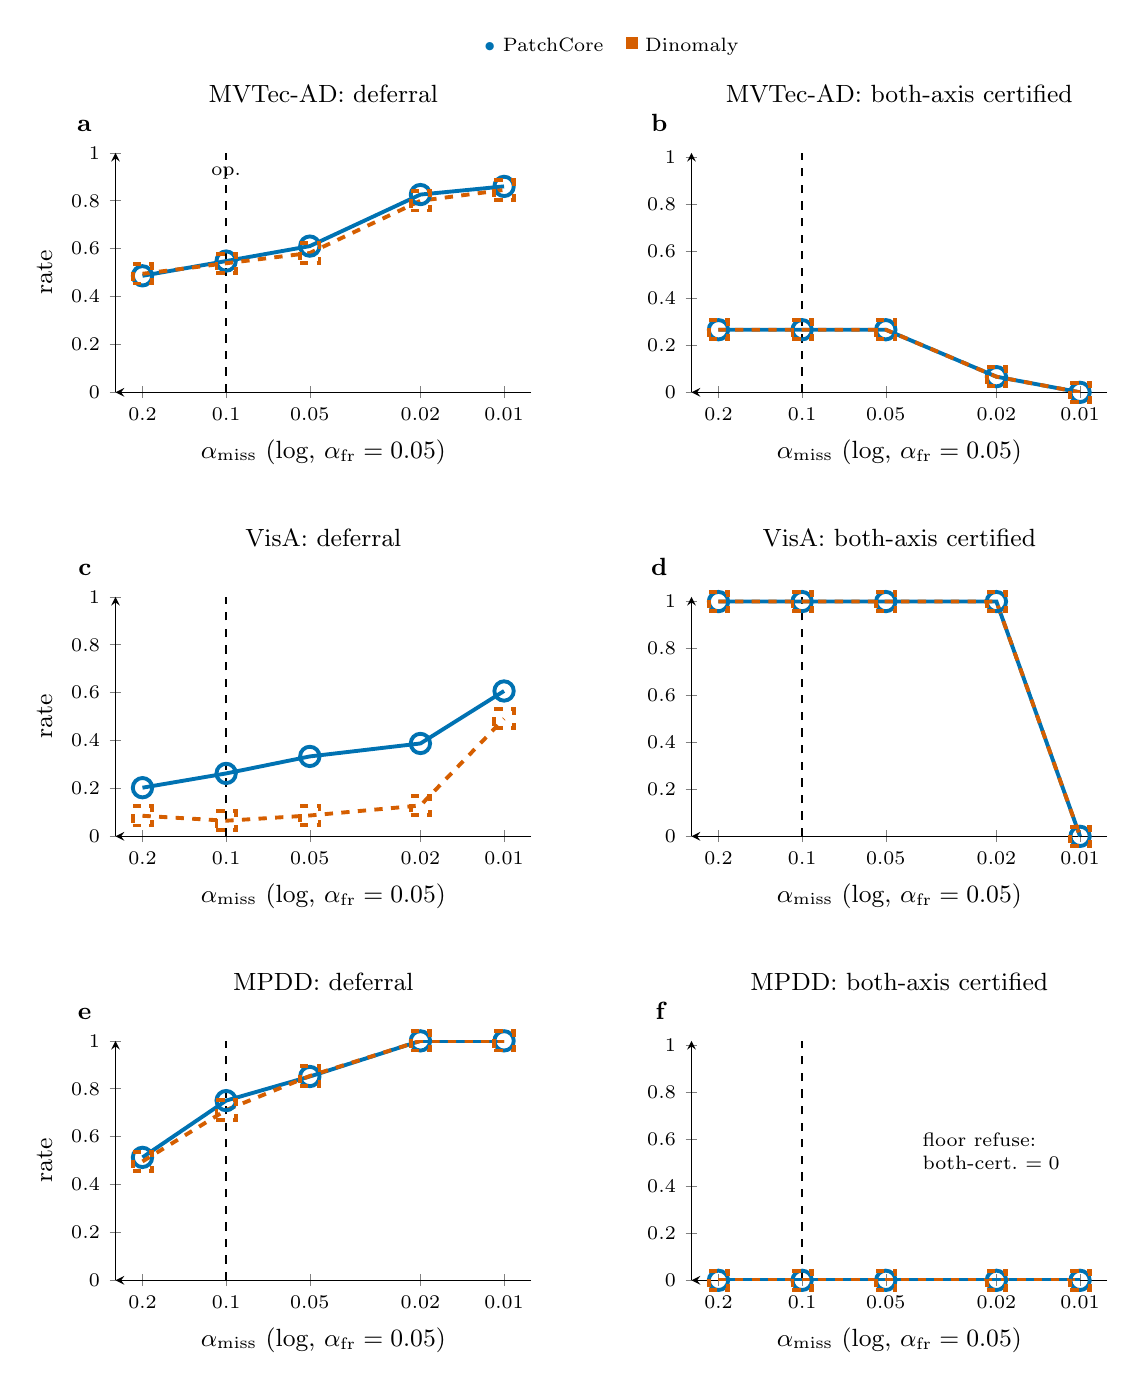
\begin{tikzpicture}[font=\figfont]

% ── MVTec-AD ────────────────────────────────────────────────────────────────
\begin{axis}[
  inspect default,
  name=ax_mvtec_d,
  width=2.70in, height=1.82in,
  at={(0.42in,4.49in)},
  xmode=log, x dir=reverse,
  xmin=0.008, xmax=0.25, ymin=0, ymax=1.0,
  xlabel={$\alpha_{\mathrm{miss}}$ (log, $\alpha_{\mathrm{fr}}=0.05$)},
  ylabel={rate},
  xtick={0.20,0.10,0.05,0.02,0.01},
  xticklabels={0.2,0.1,0.05,0.02,0.01},
  title={MVTec-AD: deferral},
]
\draw[black, dashed, line width=0.8pt] (axis cs:0.10,0) -- (axis cs:0.10,1.0);
% generated by process_alphafrontier.R
\addplot[cPatchcore, mark=o, line width=1.4pt, mark size=3.5pt] coordinates {
  (0.20,0.4866) (0.10,0.5482) (0.05,0.6106) (0.02,0.8259) (0.01,0.8600)
};
\addplot[cDinomaly, mark=square, dashed, line width=1.4pt, mark size=3.5pt] coordinates {
  (0.20,0.4951) (0.10,0.5390) (0.05,0.5818) (0.02,0.8000) (0.01,0.8454)
};

\node[anchor=north, font=\tickfont, align=center]
  at (axis cs:0.10,0.98) {op.};
\end{axis}
\panellabel{ax_mvtec_d}{a}


\begin{axis}[
  inspect default,
  name=ax_mvtec_c,
  width=2.70in, height=1.82in,
  at={(3.30in,4.49in)},
  xmode=log, x dir=reverse,
  xmin=0.008, xmax=0.25, ymin=0, ymax=1.02,
  xlabel={$\alpha_{\mathrm{miss}}$ (log, $\alpha_{\mathrm{fr}}=0.05$)},
  xtick={0.20,0.10,0.05,0.02,0.01},
  xticklabels={0.2,0.1,0.05,0.02,0.01},
  title={MVTec-AD: both-axis certified},
]
\draw[black, dashed, line width=0.8pt] (axis cs:0.10,0) -- (axis cs:0.10,1.02);
% generated by process_alphafrontier.R
\addplot[cPatchcore, mark=o, line width=1.4pt, mark size=3.5pt] coordinates {
  (0.20,0.26667) (0.10,0.26667) (0.05,0.26667) (0.02,0.06667) (0.01,0.00000)
};
\addplot[cDinomaly, mark=square, dashed, line width=1.4pt, mark size=3.5pt] coordinates {
  (0.20,0.26667) (0.10,0.26667) (0.05,0.26667) (0.02,0.06667) (0.01,0.00000)
};

\end{axis}
\panellabel{ax_mvtec_c}{b}

% Shared legend on the a/b centerline, just above the top-row titles.
% yshift 0.26in→0.44in: clear a/b titles (longer than fig-calfraction) without top clip.
\path (ax_mvtec_d.north) -- (ax_mvtec_c.north)
  coordinate[pos=0.5, yshift=0.44in] (legpos);
\node[anchor=south, font=\tickfont, text=black] (leg) at (legpos) {%
  \textcolor{cPatchcore}{$\bullet$}~PatchCore\quad
  \textcolor{cDinomaly}{\rule[0.28ex]{1.45ex}{1.45ex}}~Dinomaly%
};


% ── VisA ────────────────────────────────────────────────────────────────────
\begin{axis}[
  inspect default,
  name=ax_visa_d,
  width=2.70in, height=1.82in,
  at={(0.42in,2.27in)},
  xmode=log, x dir=reverse,
  xmin=0.008, xmax=0.25, ymin=0, ymax=1.0,
  xlabel={$\alpha_{\mathrm{miss}}$ (log, $\alpha_{\mathrm{fr}}=0.05$)},
  ylabel={rate},
  xtick={0.20,0.10,0.05,0.02,0.01},
  xticklabels={0.2,0.1,0.05,0.02,0.01},
  title={VisA: deferral},
]
\draw[black, dashed, line width=0.8pt] (axis cs:0.10,0) -- (axis cs:0.10,1.0);
% generated by process_alphafrontier.R
\addplot[cPatchcore, mark=o, line width=1.4pt, mark size=3.5pt] coordinates {
  (0.20,0.2031) (0.10,0.2627) (0.05,0.3337) (0.02,0.3878) (0.01,0.6070)
};
\addplot[cDinomaly, mark=square, dashed, line width=1.4pt, mark size=3.5pt] coordinates {
  (0.20,0.08583) (0.10,0.06516) (0.05,0.08704) (0.02,0.12880) (0.01,0.49108)
};

\end{axis}
\panellabel{ax_visa_d}{c}


\begin{axis}[
  inspect default,
  name=ax_visa_c,
  width=2.70in, height=1.82in,
  at={(3.30in,2.27in)},
  xmode=log, x dir=reverse,
  xmin=0.008, xmax=0.25, ymin=0, ymax=1.02,
  xlabel={$\alpha_{\mathrm{miss}}$ (log, $\alpha_{\mathrm{fr}}=0.05$)},
  xtick={0.20,0.10,0.05,0.02,0.01},
  xticklabels={0.2,0.1,0.05,0.02,0.01},
  title={VisA: both-axis certified},
]
\draw[black, dashed, line width=0.8pt] (axis cs:0.10,0) -- (axis cs:0.10,1.02);
% generated by process_alphafrontier.R
\addplot[cPatchcore, mark=o, line width=1.4pt, mark size=3.5pt] coordinates {
  (0.20,1) (0.10,1) (0.05,1) (0.02,1) (0.01,0)
};
\addplot[cDinomaly, mark=square, dashed, line width=1.4pt, mark size=3.5pt] coordinates {
  (0.20,1) (0.10,1) (0.05,1) (0.02,1) (0.01,0)
};

\end{axis}
\panellabel{ax_visa_c}{d}


% ── MPDD ────────────────────────────────────────────────────────────────────
\begin{axis}[
  inspect default,
  name=ax_mpdd_d,
  width=2.70in, height=1.82in,
  at={(0.42in,0.05in)},
  xmode=log, x dir=reverse,
  xmin=0.008, xmax=0.25, ymin=0, ymax=1.0,
  xlabel={$\alpha_{\mathrm{miss}}$ (log, $\alpha_{\mathrm{fr}}=0.05$)},
  ylabel={rate},
  xtick={0.20,0.10,0.05,0.02,0.01},
  xticklabels={0.2,0.1,0.05,0.02,0.01},
  title={MPDD: deferral},
]
\draw[black, dashed, line width=0.8pt] (axis cs:0.10,0) -- (axis cs:0.10,1.0);
% generated by process_alphafrontier.R
\addplot[cPatchcore, mark=o, line width=1.4pt, mark size=3.5pt] coordinates {
  (0.20,0.5134) (0.10,0.7506) (0.05,0.8512) (0.02,1.0000) (0.01,1.0000)
};
\addplot[cDinomaly, mark=square, dashed, line width=1.4pt, mark size=3.5pt] coordinates {
  (0.20,0.4964) (0.10,0.7112) (0.05,0.8534) (0.02,1.0000) (0.01,1.0000)
};

\end{axis}
\panellabel{ax_mpdd_d}{e}


\begin{axis}[
  inspect default,
  name=ax_mpdd_c,
  width=2.70in, height=1.82in,
  at={(3.30in,0.05in)},
  xmode=log, x dir=reverse,
  xmin=0.008, xmax=0.25, ymin=0, ymax=1.02,
  xlabel={$\alpha_{\mathrm{miss}}$ (log, $\alpha_{\mathrm{fr}}=0.05$)},
  xtick={0.20,0.10,0.05,0.02,0.01},
  xticklabels={0.2,0.1,0.05,0.02,0.01},
  title={MPDD: both-axis certified},
]
\draw[black, dashed, line width=0.8pt] (axis cs:0.10,0) -- (axis cs:0.10,1.02);
% generated by process_alphafrontier.R
\addplot[cPatchcore, mark=o, line width=1.4pt, mark size=3.5pt] coordinates {
  (0.20,0) (0.10,0) (0.05,0) (0.02,0) (0.01,0)
};
\addplot[cDinomaly, mark=square, dashed, line width=1.4pt, mark size=3.5pt] coordinates {
  (0.20,0) (0.10,0) (0.05,0) (0.02,0) (0.01,0)
};

% Flat zero is a measured floor refusal, not a plotting failure.
\node[anchor=west, font=\tickfont, align=left, text=black]
  at (axis cs:0.04,0.55) {floor refuse:\\ both-cert.\ $=0$};
\end{axis}
\panellabel{ax_mpdd_c}{f}


\end{tikzpicture}
\end{document}
